
\documentclass[10pt]{article} 

\usepackage[utf8]{inputenc} 
\usepackage{geometry} 
\usepackage{pgfplots,wrapfig}
\usepackage{amssymb}
\usepackage{amsmath}
\usepackage{float}
\usepackage{mathtools}
\usepackage[T1]{fontenc}

\geometry{a4paper} 
\DeclarePairedDelimiter\floor{\lfloor}{\rfloor}
\vspace{2cm}
\setlength{\parindent}{0cm}

\title{3D Camera Localization - Probabilistic Robotics}
\author{ Francesco Chichi}

\begin{document}
	\maketitle
	\section{Introduction}
		This project aims to reconstruct the poses of a vehicle, with a Least-Squares approach, using robot's odometry and anonymized observations. 
		Via G2O simulator, we obtain a landmarks based map, the robot's perceptions and the transition of the robot between two poses (the odometry).

	\section{Implementation}
		\subsection{Data Structure}
		All the project's data structures are parsed from the G2O file by the \textit{g2o\_parser} class.
		\begin{itemize}
			\item \textbf{Landmark:} This object store the position of a landmark and his ID.
			\item \textbf{Pose:} Used to represent a camera pose and his ID.
			\item \textbf{Transition:} This structure represent the transition of the robot from pose A to B. In it are stored the two poses and their relative ID.
			\item \textbf{Observation:} This kind of data structure is used to represent the robot's observations. 
			It contains the pose's ID, a vector of 2d landmarks and two vector with the relative ID and depth of each one.
			\item \textbf{DictPoints:} This dictionary is used to store match of 2D and 3D projection of a landmark.
		\end{itemize}
	
		\subsection{Camera}
		This class is used to represent a camera, initialized with the resolution (rows and columns), the camera matrix and the initial position in the space.
		It contains the two principal methods \textit{projectPoints} and \textit{unprojectPoint}, used to transform a point from 2D to 3D and vice versa.
		
		\subsection{Distance Map}
		A distance map approach is used in order to compute the data associations.
		After each transition, a distance map is computed using the G2O's observations as reference and are computed the corrispondences with the projections of the landmarks observed.

		\begin{figure}[H]
			\centering
			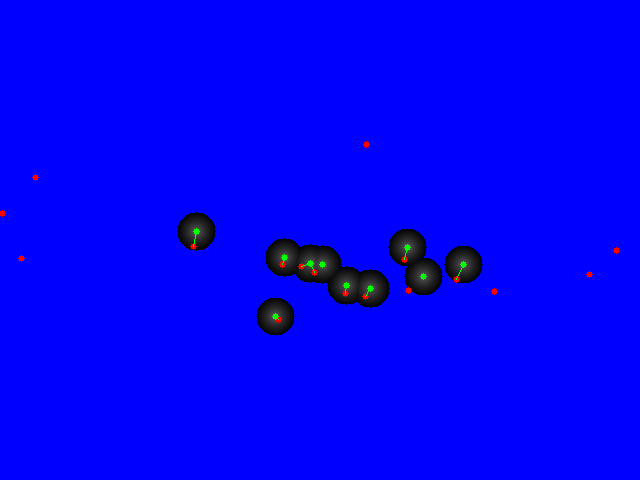
\includegraphics[width=0.7\linewidth]{img/corrispondences}
			\caption{The green points are observed points while the red are the projected landmarks.}
			\label{fig:corrispondences}
		\end{figure}

		\subsection{Main}
		The main class is used to parse the data coming out from the G2O simulation into the main data structures of the project and, for each transition of the robot, the landmarks are filtered and only those within a range are stored and used to compute the data association, in order to use correcht, using least squares, the predicted position of the camera.\\
		 		
	\section{Least-Squares Approach}
	\subsection{State}
	In the state there are the position of the camera in the space, represented as a rotation matrix and a transition vector:
	X $\in \textit{SE}(3)$ : X = (R|t)
	
	The increments $\Delta$x is represented as a ${\rm I\!R}^6$ vector: the position \textit{x},\textit{y},\textit{z} and the rotation among the three axes \textit{$\alpha_x$},\textit{$\alpha_y$},\textit{$\alpha_z$}.
	
	\subsection{Measurement}
	The measurements are the projections on the camera of the world's points.
	$z^{[\textit{m}]} \in {\rm I\!R}^2 : \textbf{z}^{[\textit{m}]} = (u^{[\textit{m}]} v^{[\textit{m}]})^T$
	
	\subsection{Prediction}
	The prediction of the camera pose at time \textit{t} is obtained applying the odometry transition at time \textit{t} to the pose \textit{t-1} \textit{($current\_camera\_pose \times cameraToRobot \times motion \times robotToCamera$)}. \\
	$h^{[\textit{n}]} = proj(K X^{-1} p^{[\textit{n}]})$.
	
	\subsection{Error}
	The error is computed as the difference between the 2D projection of the landmarks, using the predicted pose, and the observation of the same:\\
	$e^{[\textit{n,m}]} = h^{[\textit{n}]} - z^{[\textit{m}]}$
	
	\subsection{Jacobian}
	For each landmarks, the column \textit{i} of the $2\times6$ jacobian is computed using the formulae of the numerical differentiation: $ \frac{f(i +  \epsilon) - f(i-\epsilon)}{2\epsilon}$.
	
	For each landmark the procedure is the same: at the \textit{i}-th element of the state \textbf{X} are summed an $\epsilon$, then is projected the point using the modified state as reference and an error \textbf{ep} is computed as the difference between this projected point and the reference one ($z^{[\textit{m}]}$);
	The same procedure is applied subtracting the $\epsilon$, computing in this way \textbf{em}.
	
	Finally the element of the state is computed as $\frac{ep - em}{2\epsilon}$
	
	\subsection{Correction}
	The correction follows the least-squares procedure, for each least-squares iteration:
	\begin{center}
		H $\leftarrow$ H + $J_{\textit{i}}^{T}$ $\Omega_{\textit{i}}$ $J_{\textit{i}}$		
	
		b $\leftarrow$ b + $J_{\textit{i}}^{T}$ $\Omega_{\textit{i}}$ $e_{\textit{i}}$ 
	
		$\Delta x \leftarrow solve(H\Delta x=-b)$
	
		$X^* \leftarrow X^* \boxplus \Delta x$
	\end{center}
	
	\section{Front-End}
	In the \textit{Test.h} class is implemented in openCV a GUI that allows the user to visualize and navigate throw Landmarks, camera poses and transitions (figure 2). 
	
	\begin{figure}[H]
		\centering
		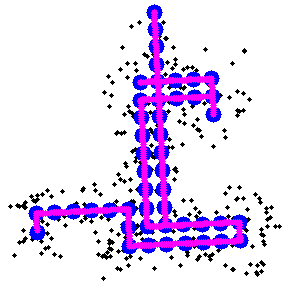
\includegraphics[width=0.5\linewidth]{img/exact}
		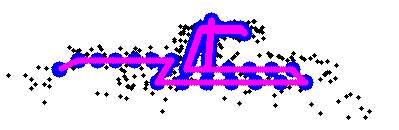
\includegraphics[width=0.8\linewidth]{img/exact2}
		\caption{The blue points are camera poses, the black ones are the landmarks and the purple are represented the transition between two poses.}
		\label{fig:exact}
	\end{figure}
	
	\section{Experimental Results}	
	Unfortunately, the purpose of the project has not been achieved. 
	
	An initially obstacle fixed was the ideal camera matrix $K_i$ gived by G2O: 
	
	\[
	K_i =
	\begin{bmatrix}
   		1 & 0 & 0.5\\
   		0 & 1 & 0.5\\
   		0 & 0 &  1
	\end{bmatrix}
	\]
	
	In order to visualize the point in the GUI, all the projected landmarks in the observations are unprojected using $K_i$ and reprojected using a camera matrix $K_r$ that have a camera focal lengths scaled by a factor \textit{scale}=150 and the optical centers centered respect to the resolution of the image:
		\[
	K_r =
	\begin{bmatrix}
   		1*scale & 0 & 0.5*cols\\
   		0 & 1*scale & 0.5*rows\\
   		0 & 0 &  1
	\end{bmatrix}
	\]
	
	Another problem fixed concerns the project "\textit{Projective Registration with unknown Associations}" seen during the lessons, where the camera is fixed at the world's center, so trasformation worldToCamera is always an identity.
In this way there are two big difference with this project:
		\begin{itemize}
			\item  Since that worldToCamera is always an identity, the $J_{icp}$ part of the jacobian becomes: $J_{icp}^{[\textit{n}]}$ = $(I_{3\times 3} | \floor{- \hat{p}^{[\textit{n}]} }_{\times})$.
			In the project the entire jacobian is computed numerically.			

			\item The projection used in the observation function uses the state X,	$h^{[\textit{n}]} = proj(K X p^{[\textit{n}]})$, because the origin of the world coincide with the camera position. In this project this semplification couldn't be done, so: $h^{[\textit{n}]} = proj(K X^{-1}. p^{[\textit{n}]})$.

		\end{itemize}
	

	
	\end{document}

